\documentclass{beamer}
\usepackage{graphicx}
\usepackage{listing}
\usepackage[utf8]{inputenc}
\usetheme{Warsaw}

\beamertemplatenavigationsymbolsempty 

\title{Bases de Datos No-SQL - Cassandra}
\author{Chapresto, Garassino, Vileriño}
\date{10 de julio de 2015}

\begin{document}

\begin{frame}
  \maketitle
\end{frame}

\begin{frame}
  \frametitle{Intro a No-SQL}    
  \framesubtitle{Porque No-SQL?}
  \begin{itemize}
    \setlength{\itemsep}{3pt}
    \item Crecimiento exponencial de dispositivos conectados a internet
    \pause
    \item Enorme cantidad de nuevos servicios prestados en la nube.
    \pause
    \item Necesidad de escalar rapidamente ante el crecimiento de la demanda.
    \pause
    \item Necesidad de alta disponibilidad, sin downtimes.
    \pause
    \item Bases de datos relacionales no funcionan del todo bien en estos contextos.
  \end{itemize}
\end{frame}

\begin{frame}
  \frametitle{Intro a No-SQL}    
  \framesubtitle{Bases de datos relacionales en problemas}
  \begin{itemize}
    \setlength{\itemsep}{3pt}
    \item Las bd relacionales son buenas para la modificacion de datos manteniendo la consistencia. 
    \pause
    \item Respetan las propiedades llamadas ACID.
    \pause
    \item Las propiedades ACID son deseables pero no siempre necesarias bajo ciertos contextos.
    \pause
    \item Cuando se comenzaron a utilizar sistemas distribuidos por los grandes volumenes de datos se not\'o que los motores relacionales no lograban desarrollar todo su potencial.
    \pause
    \item Teorema CAP: Solo se pueden tener 2 de las 3 caracteristicas: Consistencia, Disponibilidad, Tolerancia a la particion. 
  \end{itemize}
\end{frame}

\begin{frame}
  \frametitle{Intro a No-SQL}    
  \framesubtitle{Bases de datos No SQL}
  \begin{itemize}
    \setlength{\itemsep}{3pt}
    \item Surgen como solucion al problema de escalar horizontalmente
    \pause
    \item Se sacrifica en cierto grado alguna de las propiedades tradicionales(ie. Consistencia) en favor de la capacidad de escalar horizontalmente.
    \pause
    \item Se puede escalar agregando nuevos nodos \texttt{on the fly} sin perder disponibilidad(No downtime).
    \pause
    \item Principio de consistencia eventual: A pesar de que la base de datos pueda ser momentaneamente inconsistente, el estado del sistema se modificara de manera autonoma hasta converger a la consistencia.
  \end{itemize}
\end{frame}

\begin{frame}
  \frametitle{Cassandra}
  \framesubtitle{En que contextos usar Cassandra}
  \begin{itemize}
    \setlength{\itemsep}{3pt}
    \item \textbf{Arquitectura descentralizada:} No existe SPOF. Los nodos se comunican con protocolos p2p. Cada nodo puede satisfacer cualquier request.
    \pause
    \item \textbf{Replicacion a lo largo de varios data-centers: } Cassandra esta pensado para ser desplegado en un gran numero de nodos, manteniendo redundancia de datos para proveer alta disponibilidad.
    \pause
    \item \textbf{Escalable y performante: } El throughput de lecturas y escrituras aumenta linealmente con la cantidad de nodos en el sistema.
  \end{itemize}
\end{frame}

\begin{frame}
  \frametitle{Cassandra}
  \framesubtitle{En que contextos usar Cassandra}
  \begin{itemize}
    \setlength{\itemsep}{3pt}
    \item \textbf{Tolerante a fallas: } La replicacion en multiples nodos brinda resistencia ante la caida de alguno de ellos. Los nodos que fallan son reemplazables sin downtime.
    \pause
    \item \textbf{Multiples niveles de consistencia: } Lecturas y escrituras ofrecen diferentes niveles de consistencia, desde ``las escrituras jamas fallan'' hasta ``bloquear lecturas hasta tener todas las replicas'', con mecanismos de quorum \footnote{ \href{https://en.wikipedia.org/wiki/Quorum_(distributed_computing)}{Tecnicas basadas en quorum para sistemas distribuidos} Wikipedia} como punto intermedio.
    \pause
    \item \textbf{Interface legacy: } Cassandra introduce el lenguaje CQL, parecido a SQL para realizar operaciones \textbf{permitidas}(Recordar que no se pueden hacer joins por ejemplo.).
  \end{itemize}
\end{frame}




\begin{frame}
  \frametitle{Almacenamiento}
  \framesubtitle{Distribucion de los datos}
   
  \begin{itemize}
    \setlength{\itemsep}{2pt}
    \item Cassandra reparte los datos uniformemente entre los nodos de un cluster. Generalmente este conjunto de nodos es visualizado como un anillo donde cada nodo tiene vecinos.
    \pause
    \item A cada nodo se le asigna la responsabilidad sobre un rango de hashes. El rango debe configurarse de forma de distribuirlos datos de la forma mas equitativa posible. 
    \pause
    \item Cada update que se le hace a la base de datos para agregar una fila contiene una clave primaria. Esta clave es hasheada y sebusca que nodo es responsable del update.
    \pause
    \item Los nodos aprenden de la estructura general del cluster a traves deun protocolo P2P.


    \end{itemize}
\end{frame}

\begin{frame}
  \frametitle{Almacenamiento}
  \framesubtitle{Hashing}
   \begin{figure}[h!]
      \centering        
      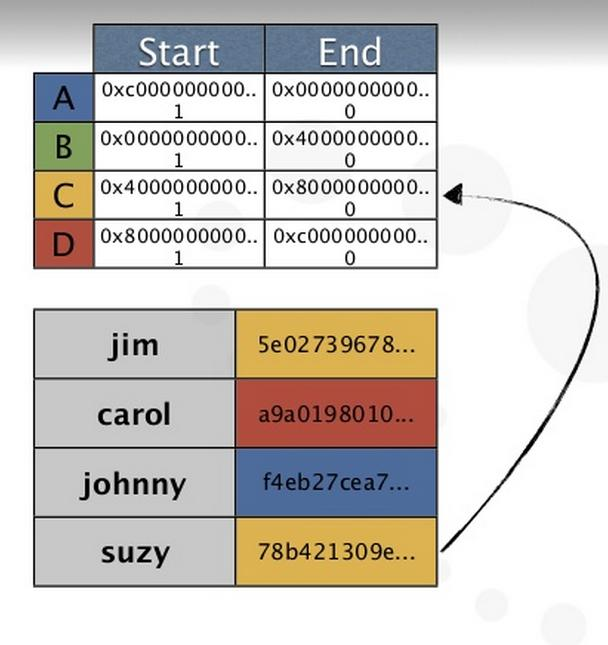
\includegraphics[scale=0.25]{hash.jpg}
      \caption{Node Hashing}
  \end{figure}

\end{frame}


\begin{frame}
  \frametitle{Almacenamiento}
  \framesubtitle{Replicacion}
   \begin{figure}[h!]
      \centering        
      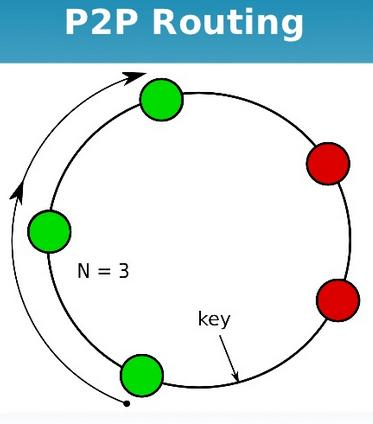
\includegraphics[scale=0.25]{p2p.jpg}
      \caption{Routeo P2P}
  \end{figure}
  \begin{itemize}
    \setlength{\itemsep}{1pt}
    \item Una vez que le llega la fila al nodo responsable, este lo replica n veces en otros nodos. Se llama n al factor de replicacion asignado a un espacio de claves. Todos los nodos son iguales y las escrituras y leturas pueden ser realizadas a traves de cualquier nodo, sea el responsable o no.
    
    \end{itemize}
\end{frame}



\begin{frame}
  \frametitle{Cassandra}
  \framesubtitle{Modelo de datos}
  \begin{itemize}
    \setlength{\itemsep}{4pt}
    \item \textbf{Implementacion: } Apache Cassandra es una base de datos NoSQL distribuida. Es de codigo abierto y esta originalmente escrita en Java.
    \pause
    \item \textbf{Modelo:} Es un hibrido entre un modelo Clave-Valor y una base de datos orientada a columnas. 
    \pause
    \item \textbf{Schemeless:} Se llama schemeless, ya que la cantidad de valores que tiene clave puede ser totalmente distinta a la de las demas.
  \end{itemize}
\end{frame}
  

\begin{frame}
  \frametitle{Cassandra-Modelo}
  \framesubtitle{Columna}
   \begin{figure}[h!]
      \centering        
      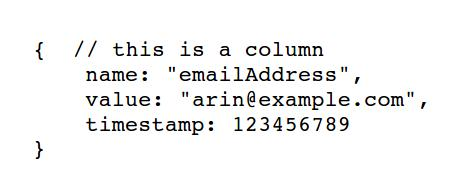
\includegraphics[scale=0.4]{column.jpg}
      \caption{Columna}
  \end{figure}

  \begin{itemize}
    \setlength{\itemsep}{4pt}
    \item La \textbf{columna} es a minima unidad de almacenamiento. Es una tripla, con nombre, valor y un timestamp.
    \pause
    \item  Los tres campos son tipos primitivos. 
    \pause
    \item  Para simplificarde ahora en adelante, ignoramos el timestamp, para poder pensarlo como un par (valor, nombre).
    
    

  \end{itemize}
\end{frame}


\begin{frame}
  \frametitle{Cassandra-Modelo}
  \framesubtitle{SuperColumna}
   \begin{figure}[h!]
      \centering        
      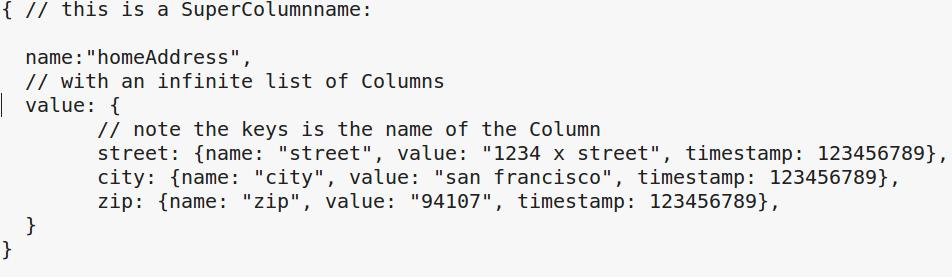
\includegraphics[scale=0.25]{supercolumn.jpg}
      \caption{SuperColumna}
  \end{figure}

  \begin{itemize}
    \setlength{\itemsep}{2pt}
    \item La \textbf{SuperColumna} es una tupla con un nombre de tipo primitivo y un valor.
    \pause
    \item La diferencia con una columna, es que el valor, en lugar de ser un tipo primitivo, es un conjunto de columnas indexadas por el nombre de cada una.
    \pause
    \item Ademas, tampoco poseen un timestamp. Por lo que pueden pensarse como tuplas, (nombre, diccionarioDeColumnas).
  \end{itemize}
\end{frame}

\begin{frame}
  \frametitle{Cassandra-Modelo}
  \framesubtitle{Familia de Columna}
   \begin{figure}[h!]
      \centering        
      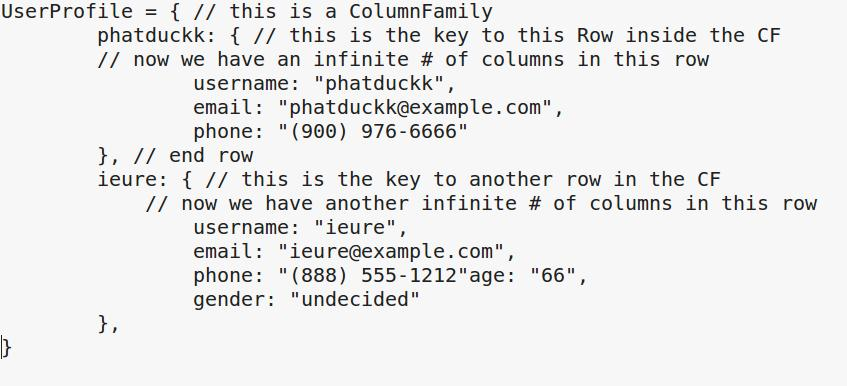
\includegraphics[scale=0.25]{familia.jpg}
      \caption{Familia de Columna}
  \end{figure}

  \begin{itemize}
    \setlength{\itemsep}{2pt}
    \item La \textbf{Familia de Columna} es una estructura que agrupa columnas y supercolumnas. Se puede pensar como una tabla de RDMB.
    \pause
    \item Tiene un nombre y \textbf{Filas}, que, pensando en RDBM, serian los registros de una tabla.
    \pause
    \item Las filas se indexan con una clave que provee el usuario, y poseen un conjunto de columnas o supercolumnas indexadas por sus nombres. (En el ejemplo, son solo columnas)
    \item No poseen un esquema. Las filas pueden tener diferentes columnas y numero de ellas
  \end{itemize}
\end{frame}


\begin{frame}
  \frametitle{Cassandra-Modelo}
  \framesubtitle{SuperFamilia de Columna}
   \begin{figure}[h!]
      \centering        
      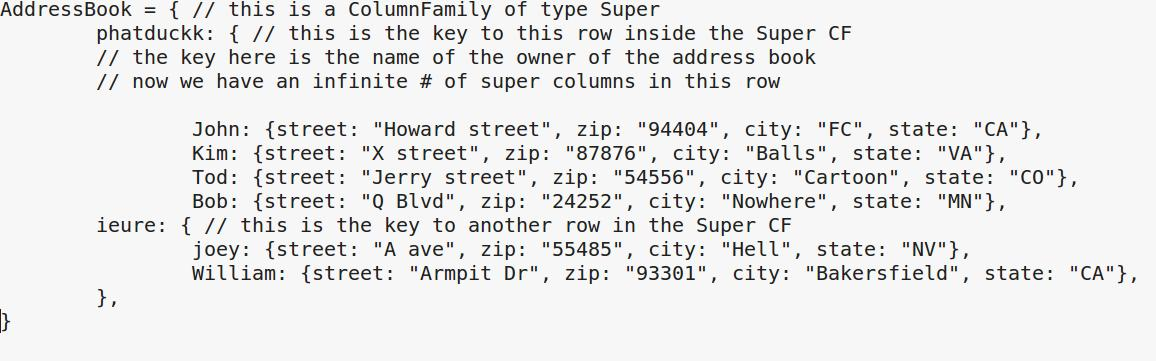
\includegraphics[scale=0.25]{superfamily.jpg}
      \caption{SuperFamilia de Columna}
  \end{figure}

  \begin{itemize}
    \setlength{\itemsep}{2pt}
    \item La \textbf{SuperFamilia de Columna} es una familia de supercolumnas.
    \pause
    \item Posee un conjunto de filas que son superColumnas indexadas por su nombre, cada una de ellas tiene un conjunto de columnas
    \pause
    \item Tampoco poseen esquema fijo.
  \end{itemize}
\end{frame}


\begin{frame}
  \frametitle{Cassandra-Modelo}
  \framesubtitle{Espacio de claves}
   
  \begin{itemize}
    \setlength{\itemsep}{4pt}
    \item El \textbf{Espacio de claves} es el agrupamiento mas externo delos datos. Ahi se almacenan todas las SuperFamilias de columnas.
    \pause
    \item Puede no haber ninguna relacion entre las familias de columnas. 
    \item No son tablas de SQL, no se pueden joinear, ya que pueden no tener ni una columna en comun.
    \end{itemize}
\end{frame}



\begin{frame}
  \frametitle{Sorting}
  \framesubtitle{Ordenamiento de los datos}
   
  \begin{itemize}
    \setlength{\itemsep}{4pt}
    \item En Cassandra, no puede especificarse el orden en que se quieren ordenados los datos que se consultan.
    \pause
    \item Los datos se ordenan en el momento de la insercion y quedan ordenados. 
    \pause
    \item Esto da una mejora de perfomance en las lecturas, pero el modelo de datos debe planificarse acordemente de
    forma de poder satisfacer los patrones de acceso.
    \item Dentro de su fila, las columnas estan ordenadas por su nombre. La funcion que compara los nombres se define dentro de cada superfamilia.
    \end{itemize}
\end{frame}

 
\begin{frame}
  \frametitle{Sorting}
  \framesubtitle{Ordenamiento de los datos}
   
  \begin{itemize}
    \setlength{\itemsep}{2pt}
    \item Este modelo simple y desestructurado tiene sus desventajas.
    \pause
    \item Por ejemplo, para ordenar por un determinado campo, es necesario que forme parte de la clave (nombre) de la fila. 
    \pause
    \item Cuando la clave esta compuesta por multiples elementos se denomina clave compuesta, y se divide en dos partes: la partition key y la clustering key.
    \pause
    \item La partition key es la minima cantidad de datos que hay que proveer en una consulta para obtener las filas deseadas. La clustering key, son datos extra que sirven por ejemplo para aprovechar las capacidades de ordenamiento.
    \end{itemize}
\end{frame}


\end{document}